\section{Definición}

Una de las categorías protagonistas de la geometría compleja es la categoría de las \textit{variedades compleja}. Los objetos que estudiaremos serán espacios Hausdorff que se modelan localmente como abiertos de $\cc^n$ y esto permite extender los conceptos del análisis complejo clásico a un contexto de geometría global.

\begin{definition}
	Sea $M$ un espacio topológico Hausdorff y segundo numerable. Decimos que $M$ es una \textbf{variedad compleja} (de dimensión $n$) si existe un par $\{(U_i,\varphi_i)\}$ tales que
	\begin{enumerate}
		\item $\{U_i\}_{i\in I}$ es una cubierta abierta de $M$.
		\item Para cada $i\in I$, se tiene que $\varphi_i:U_i\to\varphi_i(U_i)\subset \cc^n$ es un homeomorfismo.
		\item Para cada $i,j\in I$, si $U_i\cap U_j\neq\emptyset$ entonces la aplicación
		\begin{equation*}
			\varphi_{ij}=\varphi_j\circ\varphi_i^{-1}:\varphi_i(U_i\cap U_j)\to\varphi_j(U_i\cap U_j),
		\end{equation*}
		llamada \textbf{función de transición}, es holomorfa.
		\begin{figure}[H]
			\centering
			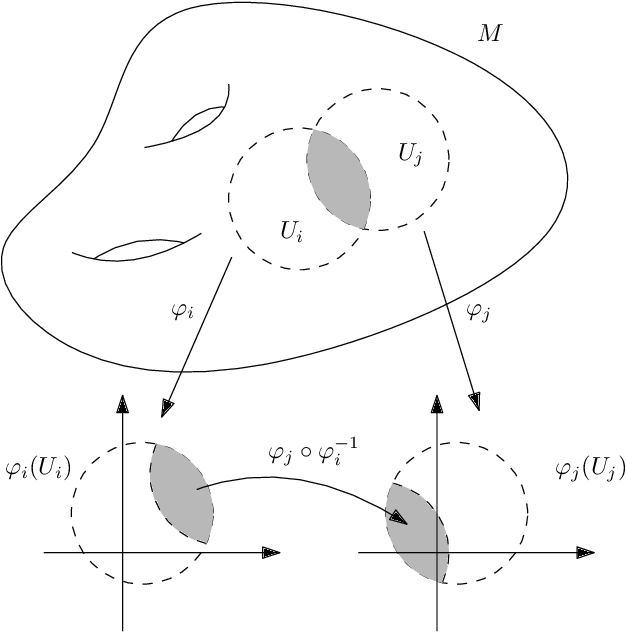
\includegraphics[width=0.3\linewidth]{Imagenes/atlas holomorfo}
			\caption{Representación de cartas holomorfa.}
			\label{fig:atlas-holomorfo}
		\end{figure}
		
	\end{enumerate}
	El par $(U_i,\varphi_i)$ es llamado \textbf{carta holomorfa} y la colección $\{(U_i,\varphi_i)\}$ de todas las cartas es llamado \textbf{atlas holomorfo}. Si existe un atlas holomorfo para $M$, también vamos a decir que \textbf{admite una estructura analítica}.
	Una \textbf{curva compleja} es una variedad compleja de dimensión $1$, y si además es conexa le llamamos \textbf{superficie de Riemann}. Por último, decimos que una variedad compleja de dimensión $2$ es una \textbf{superficie compleja}.
\end{definition}


\subsection{Ejemplos}
Ahora vamos a presentar varios ejemplos esenciales de variedades complejas.


\begin{example}[$ n $-espacio afín $\cc^n$]   
	Consideremos el espacio complejo $\cc^n$. Un atlas holomorfo para este espacio está dado por $\mathscr{A}=\{(\cc^n,\mathrm{id})\}$\footnote{Note que no es un atlas maximal.}, además de cumplir con todas las propiedades topológicas que necesitamos para ser una variedad compleja. Este será nuestro ejemplo base de variedad compleja no compacta. 
\end{example}

\begin{example}[Abierto de una variedad]
	Si $M$ es una variedad compleja con atlas holomorfo $\{(U_i,\varphi_i)\}$, entonces todo abierto no vacío $U\subset M$ es una variedad compleja con atlas holomorfo $\{(U\cap U_i,\varphi_i|_{U\cap U_i})\}$.
\end{example}

\begin{example}[Producto de variedades]
	Si $M_1,\dots, M_k$ son variedades complejas de dimensión $n_1,\dots,n_k$ respectivamente. Entonces el producto $M_1\times \cdots\times M_k$ es una variedad compleja de dimensión $n_1+\cdots+n_k$ cuyas cartas son de la forma $(U_1\times\cdots\times U_k,\varphi_1\times\cdots\times \varphi_k)$. Notemos que las cartas son compatibles pues
	\begin{equation*}
		(\psi_1\times\cdots\times \psi_k)\circ (\varphi_1\times\cdots\times \varphi_k)^{-1}=(\psi_1\circ\varphi_1^{-1})\times\cdots\times (\psi_k\circ \varphi_k^{-1})
	\end{equation*}
	es una aplicación holomorfa.
\end{example}

\begin{example}[Toro Complejo]
	Consideremos $V$ un $\cc$-espacio vectorial de dimensión $n$. Una \textbf{retícula} en $V$ es un subgrupo aditivo abeliano discreto $\Lambda\subset V$ generada por $2n$ vectores $v_1,\cdots,v_{2n}$ los cuales son linealmente independientes sobre $\rr$. El cociente $V/\Lambda$ es una variedad compleja de dimensión $n$ compacta y conexa (véase \parencite[Example 1.18]{leecomplex}). Además, se puede determinar un difeomorfismo entre $V/\Lambda$ y el producto de círculos $(S^1)^{2n}$.
	Un caso particularmente interesante es el cociente 
	\begin{equation*}
		T=\cc/\Lambda
	\end{equation*}
	donde $\Lambda=w_1\zz+w_2\zz$ y $w_1,w_2$ son linealmente independientes sobre $\rr$. Esta curva compleja es llamada \textbf{curva elíptica}.
	\begin{figure}[H]
		\centering
		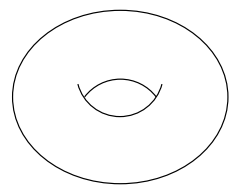
\includegraphics[width=0.25\linewidth]{Imagenes/toro}
		\caption{Modelo topológico de las curvas elípticas.}
		\label{fig:toro}
	\end{figure}
\end{example}

    \begin{example}[Variedades de Hopf]
	    	Consideremos $\lambda=(\lambda_1,\dots,\lambda_n)$ una $n$-tupla ordenada de números reales tal que $0<\lambda_i<1$, y definamos la acción $\cdot:\zz\times\cc^n\setminus\{0\}\to\cc^n\setminus\{0\}$ dada por
	    	\begin{equation*}
		    		k\cdot z=((\lambda_1)^kz_1,\dots,(\lambda_n)^kz_n).
		    	\end{equation*}
	    	Esta acción es holomorfa, libre y propia, por lo que el cociente bajo esta acción
	    	\begin{equation*}
		    		H=\frac{\cc^n\setminus\{0\}}{\zz}
		    	\end{equation*}
	    	es una variedad compleja conexa y compacta llamada \textbf{variedad de Hopf}. Más aún, esta variedad $H$ es difeomorfa a $S^{2n-1}\times S^1$. (veáse \parencite[Example 1.19]{leecomplex})
	    \end{example}

Ahora vamos a ver con detalle cómo los ceros de funciones holomorfas determinan variedades complejas. Lo anterior es fundamental para determinar la estructura analítica de las variedades algebraicas, pues los polinomios son funciones holomorfas.

\begin{example}[Hipersuperficie afín]
	Consideremos una función holomorfa $f:\cc^n\to \cc$ con $0\in\cc$ un valor regular. Sea
	\begin{equation*}
		X:=f^{-1}(0)=Z(f)\subset \cc^n
	\end{equation*}
	y $p\in X$. Escribiendo $f=f(z_1,\dots,z_n)$, el jacobiano de $f$ en $p$ está dado por
	\begin{equation*}
		J(f)(p)=\left(\frac{\partial f}{\partial z_1}(p),\dots, \frac{\partial f}{\partial z_n}(p)\right).
	\end{equation*}
	Como $0\in\cc$ es un valor regular, entonces $p$ es un punto regular. Así, el rango de la matriz $J(f)(p)$ (de tamaño $1\times n$) es $1$, es decir, al menos una derivada parcial no se anula en $p$. Sin pérdida de generalidad, podemos asumir que 
	\begin{equation*}
		\frac{\partial f}{\partial z_n}(p)\neq 0.
	\end{equation*}
	En particular, existe una vecindad $U\subset\cc^n$ de $p$ donde $\frac{\partial f}{\partial z_n}$ no se anula. Renombrando las coordenadas $w=(z_1,\dots,z_{n-1})$ y $z=z_n$, se puede escribir $f=f(w,z)$. Por el teorema de la función implícita \ref{funcionimplicita}, existe una vecindad $W\subset\cc^{n-1}$ de $w_0=(p_1,\dots,p_{n-1})$ y una función holomorfa $g:W\to\cc$ tal que $f(w,g(w))=0$ para todo $w\in W$ y  
	\begin{equation*}
		\{(w,z)\in W\times\cc:f(w,z)=0\}=\{(w,g(w)):w\in W\}.
	\end{equation*}
	Definamos ahora la función
	\begin{align*}
		\varphi:X\cap U&\longrightarrow W\subset\cc^{n-1}\\
		(w,z)&\longmapsto w.
	\end{align*}
	\begin{center}
		\begin{figure}[H]
			\centering
			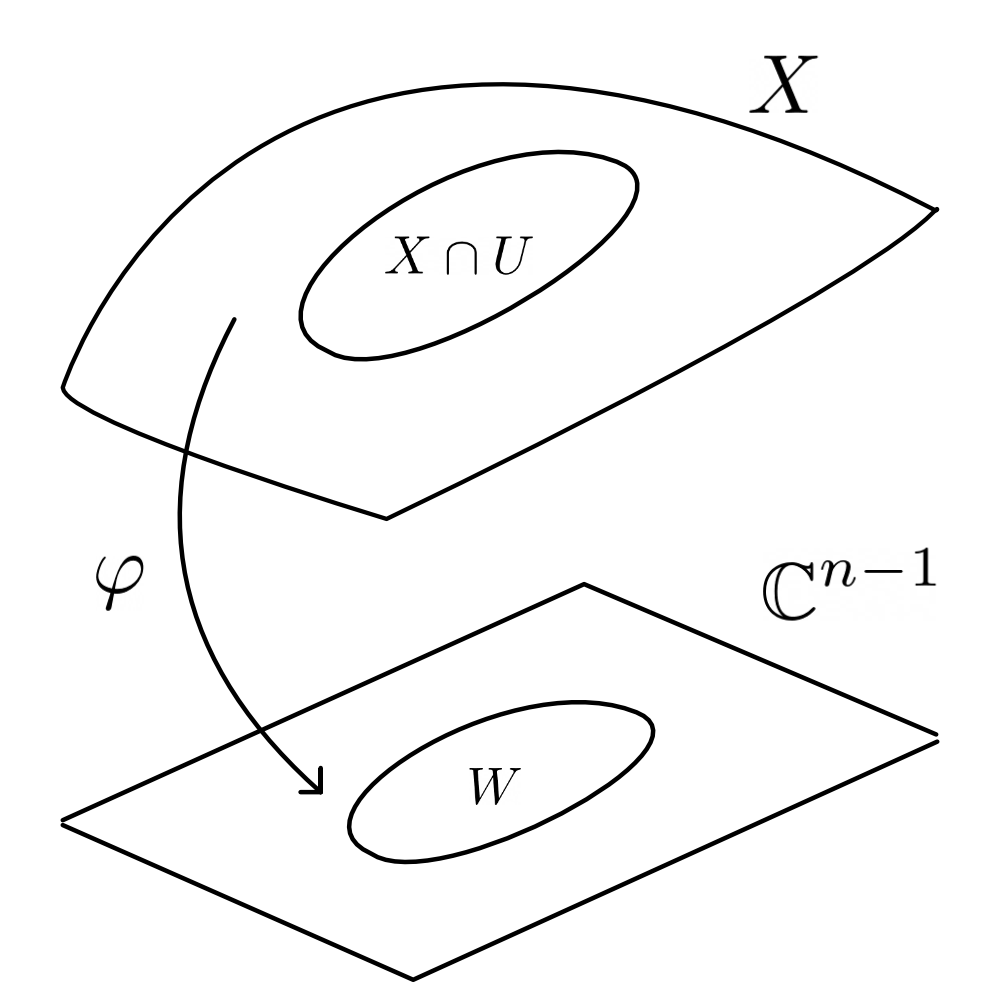
\includegraphics[width=0.3\linewidth]{Imagenes/hipersuperficie afin}
			\caption{Carta de la hipersuperficie afín.}
			\label{fig:hipersuperficie-afin}
		\end{figure}
	\end{center}
	Queremos ver que $\varphi$ es una carta para $p$. Probemos primero que es inyectiva y sobreyectiva.
	\begin{itemize}
		\item Sean $x,x'\in X\cap U$ tales que $\varphi(x)=\varphi(x')$. Si $x=(w,z)$ y $x'=(w',z')$, entonces $z=g(w)$ y $z'=g(w')$. Así,
		\begin{align*}
			\varphi(x)&=\varphi(x')\\
			w&=w'
		\end{align*}
		De esta forma, $z=z'$ y por tanto $x=x'$. Esto significa que $\varphi$ es inyectiva.
		\item Sea $w\in W$, entonces $(w,g(w))\in X\cap U$ y
		\begin{equation*}
			\varphi(w,g(w))=w.
		\end{equation*}
		Así, $\varphi$ es sobreyectiva.
	\end{itemize}
	Con esto, $\varphi$ es biyectiva y además la inversa de $\varphi$ está dada por
	\begin{align*}
		\varphi^{-1}:W\to X\cap U\\
		w\mapsto (w,g(w))
	\end{align*}
	
	Como $\varphi$ y $\varphi^{-1}$ son aplicaciones holomorfas, en particular son funciones continuas.
	Dado que todo punto de $X$ es regular, para cada $p\in X$ existe un abierto $U$ y una carta centrada en $p$. Ahora probemos que las funciones de transición son holomorfas.\\
	Sea $p\in X\cap U$ otro punto con carta $\psi:X\cap U'\to W'$, entonces
	\begin{equation*}
		\psi\circ\varphi^{-1}:\varphi((X\cap U)\cap(X\cap U'))\to\psi((X\cap U)\cap(X\cap U'))
	\end{equation*}
	es una función tal que 
	\begin{equation*}
		w\mapsto (w',g(w'))\mapsto w'
	\end{equation*}
	donde $w'$ es la proyección sobre las $n-1$ coordenadas elegidas por la carta $\psi$. Dado que ambas proyecciones son holomorfas, entonces la función de transición $\psi\circ\varphi^{-1}$ es holomorfa. Como $\varphi^{-1}$ está dada por $(w,g(w))$ y $\psi$ es una proyección de coordenadas, la composición $\psi\circ\varphi^{-1}$ es holomorfa.
	De esta manera, las cartas $(X\cap U,\varphi)$ dotan a $X$ de un atlas holomorfo.\\
	Más aún, $X$ como subespacio de $\cc^n$ es un espacio Hausdorff, segundo numerable y con estructura holomorfa. Por lo tanto, $X$ es una variedad compleja de dimensión $n-1$.
\end{example}

Generalizando este último ejemplo tenemos:
\begin{example}[Intersección compleja]\label{interseccioncompleja}
	Sean $k$ funciones holomorfas $f_1,f_2,\cdots,f_k:\cc^n\to \cc$, con $k\leq n$ y definamos la aplicación holomorfa asociada
	\begin{equation*}
		f=(f_1,\dots,f_k):\cc^n\to\cc^k.
	\end{equation*}   
	Supongamos que $0\in\cc^k$ es un valor regular de $f$. Entonces el conjunto
	\begin{equation*}
		X:=f^{-1}(0)=Z(f_1)\cap\cdots\cap Z(f_k)=Z(f_1,\dots,f_k)
	\end{equation*}
	es una variedad compleja de dimensión $n-k$.\\
	La demostración sigue la misma estrategia para el caso $k=1$ con ciertas observaciones:
	\begin{itemize}
		\item Para cada punto $p\in X$, el rango de la matriz jacobiana $J(f)(p)$ es $k$. Por una renumeración de las variables, podemos suponer que la submatriz cuadrada de las últimas $k$ variables tiene determinante no cero.
		\item Por el teorema de la función implícita, tenemos una vecindad $W\subset\cc^{n-k}$ de las primeras $n-k$ entradas de $p$, una vecindad $Z\subset\cc^k$ de las últimas $k$ entradas de $p$ y una aplicación holomorfa
		\begin{equation*}
			g:W\to Z
		\end{equation*}
		\item Las cartas $\varphi:X\cap U\to W\subset\cc^{n-k}$ se construyen de la misma manera y la transición sigue siendo holomorfa como antes, por componerse de proyecciones y las funciones holomorfas $g$.
	\end{itemize}
	
\end{example}

\begin{example}[Espacio proyectivo]
	El \textbf{n-espacio proyectivo} es el conjunto $\pp^n=\cc^{n+1}\setminus\{0\}/\sim$ donde $z,w\in\cc^{n+1}\setminus\{0\}$ están relacionados si, y solo si, existe $\lambda\in\cc\setminus\{0\}$ tal que  $z=\lambda w$.
	
	Dotamos a $\pp^n$ con la topología cociente dada por la proyección canónica
	\begin{equation*}
		q:\cc^{n+1}\setminus \{0\} \longrightarrow \pp^n
	\end{equation*}
	Consideremos la cubierta estándar afín de $\pp^n$ dada por los $n+1$ abiertos
	\begin{equation*}
		U_i=\{[x_0:\cdots:x_n]:x_i\neq 0\}\subset \pp^n
	\end{equation*}
	Así, tenemos las funciones $\varphi_i:U_i\to\cc^n$ dadas por
	\begin{align*}
		[x_0:x_1:\dots:x_n]\mapsto & \left( \frac{x_0}{x_i},\frac{x_1}{x_i},\dots, \frac{x_{i-1}}{x_i},\frac{x_{i+1}}{x_i},\dots,\frac{x_n}{x_i}\right)
	\end{align*} 
	Estas funciones son continuas por la propiedad característica de la topología cociente y su inversa está dada por
	\begin{equation*}
		\varphi_{i}^{-1}(z_1,\dots,z_n)=[z_1:\dots:z_{i-1}:1:z_{i+1}:\dots:z_n]
	\end{equation*}
	Así, las funciones $\varphi_i$ son homeomorfismos llamados \textbf{cartas afines}.
	Además, las funciones de transición $\varphi_{ij}=\varphi_i\circ\varphi_j^{-1}:\varphi_j(U_i\cap U_j)\to\varphi_i(U_i\cap U_j)$ están dadas por
	\begin{equation*}
		\varphi_{ij}(w_1,\dots,w_n)=\left(\frac{w_1}{w_i},\dots \frac{w_{i-1}}{w_i},\frac{w_{i+1}}{w_i},\dots,\frac{w_{j-1}}{w_i},\frac{1}{w_i},\frac{w_{j+1}}{w_i},\dots,\frac{w_n}{w_i} \right)
	\end{equation*}
	Notemos que $\varphi_i(U_i \cap U_j)=\cc^n\setminus Z(w_j)$. Con esto, las funciones $\varphi_{ij}$ son aplicaciones holomorfas.\\
	Las propiedades topológicas de Hausdorff y segundo numerable son análogas al caso de $\pp^1$ (véase \parencite[Cap. 1, Sec. 1, Ejem. 1.3]{zaldrimann}).\\
	Si consideramos la esfera $S^{2n+1}$ unitaria de $\cc^{n+1}$, entonces tenemos la siguiente composición de funciones continuas\footnote{A la tríada $(S^{2n+1},q,\pp^n)$ se le llama \textbf{fibrado de Hopf}.}
	\[\begin{tikzcd}
		{S^{2n+1}} && {\cc^{n+1}\setminus\{0\}} \\
		\\
		&& {\mathbb{P}^n}
		\arrow[hook, from=1-1, to=1-3]
		\arrow["\rho"', dashed, from=1-1, to=3-3]
		\arrow["p", two heads, from=1-3, to=3-3]
	\end{tikzcd}\]
	Como $\pp^n$ es la imagen continua de $S^{2n+1}$ bajo $\rho$ y la esfera es conexa y compacta, entonces podemos concluir que el espacio proyectivo $\pp^n$ es conexo y compacto.
	Por lo tanto, $\pp^n$ es una variedad compleja conexa y compacta.
\end{example}
\begin{figure}[H]
	\centering
	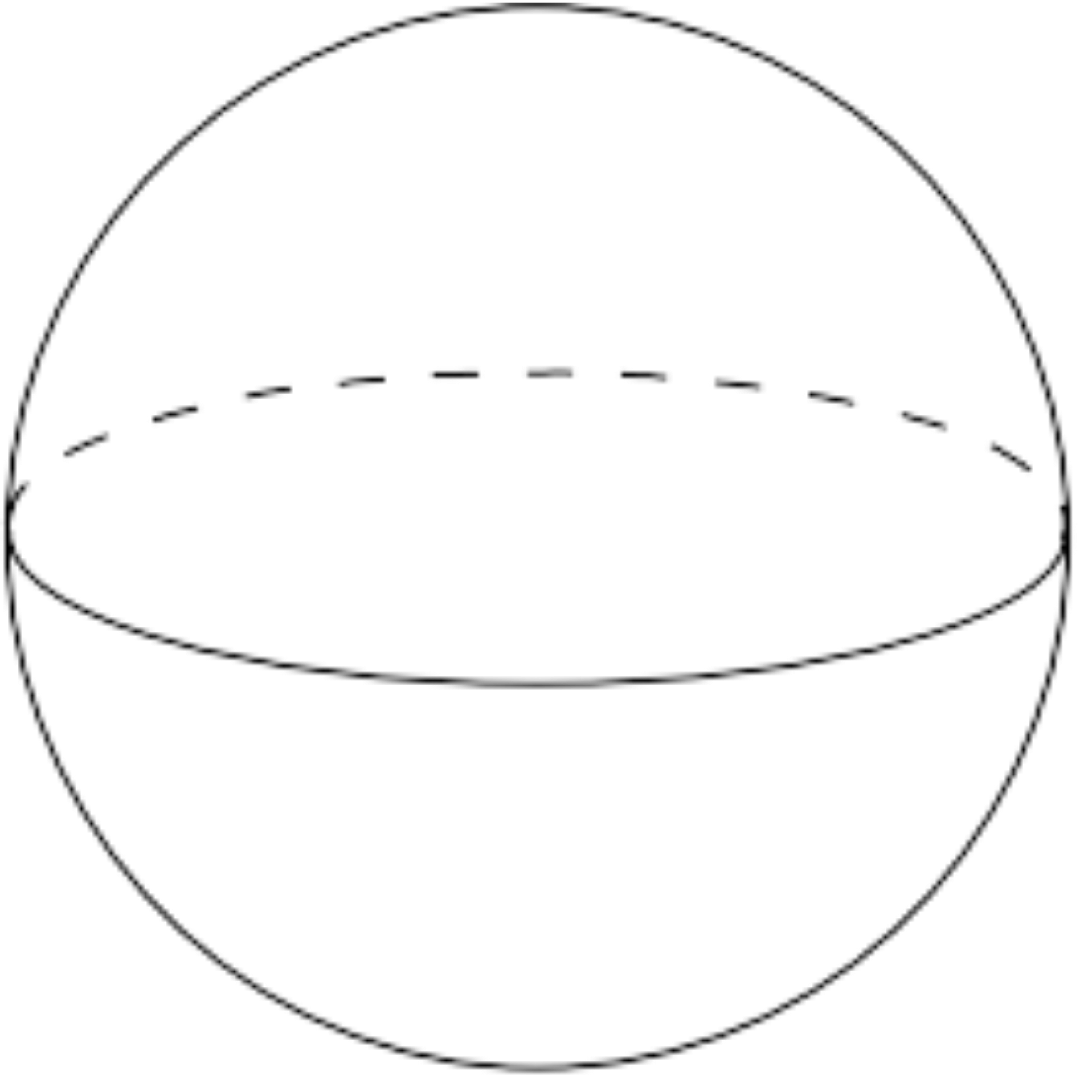
\includegraphics[width=0.2\linewidth]{Imagenes/Esfera}
	\caption{Recta proyectica $\pp^1$}
	\label{fig:esfera}
\end{figure}

En este trabajo nos enfocaremos principalmente en las variedades compactas conexas, pues muchos resultados importantes se sustentan bajo estas hipótesis y son esenciales para el tema de algebrización. Veremos con más detalle esto último en el segundo capítulo.

\subsection{La esfera de Riemann}

Aquí desarrollaremos tres ejemplos de superficies de Riemann que pueden verse distintos, pero que en esencia serán la misma superficie. Especificamente hablamos de la esfera unitaria en $\rr^3$, el plano extendido $\overline{\cc}:=\cc\cup \{\infty\}$ y la recta proyectiva compleja $\pp^1$. Es conocido que topológicamente estos espacios son homeomorfos y por consecuencia superficies de género $0$ (falta cita). Sin embargo, veremos que sus estructuras holomorfas serán también compatibles. Siendo exactos, estos tres espacios serán biholomorfos (falta cita).

\begin{example}[Esfera de Riemann]
	Considere la esfera unitaria en $\rr^3$ dada por
	\begin{equation*}
		S^2=\{(x_1,x_2,x_3)\in\rr^3:x_1^2+x_2^2+x_3^2=1\}
	\end{equation*}
	Podemos dotar a $S^2$ con la topología del subespacio y de esta manera $S^2$ es conexo, Hausdorff y segundo numerable.
	\begin{figure}[H]
		\centering
		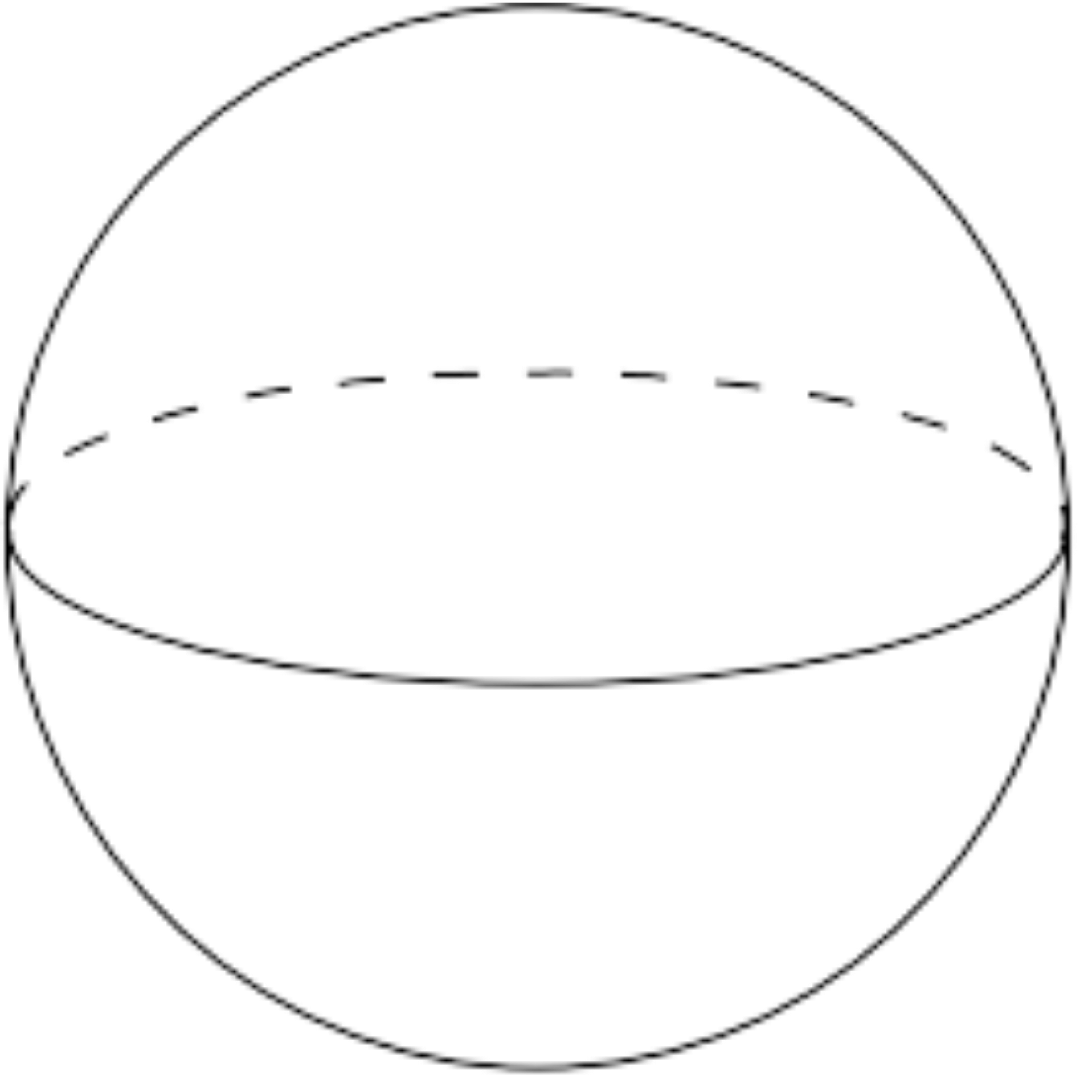
\includegraphics[width=0.25\linewidth]{Imagenes/Esfera.png}
		\caption{Esfera de Riemann \cite[Fig. 10.1, p. 170]{Sambarino}}
	\end{figure}
	Definamos la cubierta
	\begin{equation*}
		U_0=S^2\setminus(0,0,1),\qquad U_1=S^2\setminus(0,0,-1)
	\end{equation*}
	y las funciones 
	\begin{equation*}
		\varphi_0:U_0\to\cc,\qquad \varphi_1:U_1\to\cc
	\end{equation*}
	dadas por
	\begin{equation*}
		\varphi_0(x_1,x_2,x_3)=\frac{x_1}{1-x_3}+i\frac{x_2}{1-x_3},\qquad \varphi_1(x_1,x_2,x_3)=\frac{x_1}{1+x_3}-i\frac{x_2}{1+x_3}
	\end{equation*}
	Note que las funciones son continuas por criterio por componentes.\\
	Además, se puede determinar que $\varphi^{-1}_0:\cc\to U_0$ y $\varphi^{-1}_1:\cc\to U_1$ dadas por
	\begin{equation*}
		\varphi^{-1}_0(z)=\left( \frac{2\mathrm{Re}(z)}{1+|z|^2},\frac{2\mathrm{Im}(z)}{1+|z|^2},\frac{1-|z|^2}{1+|z|^2} \right)\qquad \varphi^{-1}_1(z)=\left( \frac{2\mathrm{Re}(z)}{1+|z|^2},-\frac{2\mathrm{Im}(z)}{1+|z|^2},\frac{1-|z|^2}{1+|z|^2} \right)
	\end{equation*}
	Luego, $U_0\cap U_1=S^2\setminus\{(0,0,1),(0,0,-1)\}$. Si $z\in \cc\setminus\{0\}$, entonces
	\begin{equation*}
		\left( \frac{2\mathrm{Re}(z)}{1+|z|^2},\frac{2\mathrm{Im}(z)}{1+|z|^2},\frac{1-|z|^2}{1+|z|^2} \right)\in U_0\cap U_1
	\end{equation*}
	y 
	\begin{equation*}
		\varphi_0\left( \frac{2\mathrm{Re}(z)}{1+|z|^2},\frac{2\mathrm{Im}(z)}{1+|z|^2},\frac{1-|z|^2}{1+|z|^2} \right)=z
	\end{equation*}
	De esta manera, $\varphi_0(U_0\cap U_1)=\cc\setminus\{0\}$. Análogamente, $\varphi_1(U_0\cap U_1)=\cc\setminus\{0\}$.\\
	Así, $\varphi_0(U_0\cap U_1)=\varphi_1(U_0\cap U_1)$ es un abierto en $\cc$ (por ser complemento de un conjunto unipuntual).\\
	Considerando la función de transición
	\begin{equation*}
		\varphi_{01}=\varphi_0\circ \varphi_1^{-1}:\varphi_1(U_0\cap U_1)\to\varphi_0(U_0\cap U_1)
	\end{equation*}
	se tiene que
	\begin{align*}
		\varphi_0\circ \varphi_1^{-1}(z)&=\varphi_0\left( \frac{2\mathrm{Re}(z)}{1+|z|^2},-\frac{2\mathrm{Im}(z)}{1+|z|^2},\frac{1-|z|^2}{1+|z|^2} \right)\\
		&=\frac{\frac{2\mathrm{Re}(z)}{1+|z|^2}}{1-\frac{1-|z|^2}{1+|z|^2}}+i\frac{-\frac{2\mathrm{Im}(z)}{1+|z|^2}}{1-\frac{1-|z|^2}{1+|z|^2}}\\
		&=\frac{2\mathrm{Re}(z)}{2|z|^2}-i\frac{2\mathrm{Im}(z)}{2|z|^2}\\
		&=\frac{\mathrm{Re}(z)-\mathrm{Im}(z)i}{|z|^2}\\
		&=\frac{\mathrm{Re}(z)-\mathrm{Im}(z)i}{(\mathrm{Re}(z)-\mathrm{Im}(z)i)(\mathrm{Re}(z)-\mathrm{Im}(z)i)}\\
		&=\frac{1}{z}
	\end{align*}
	la cual está bien definida ya que $\varphi_1(U_0\cap U_1)=\cc\setminus\{0\}$. Además, es holomorfa en todo su dominio.\textbf{Aquí una imagen}\\
	Esto implica que $\mathscr{A}=\{(U_0,\varphi_0),(U_1,\varphi_1)\}$ es un atlas holomorfo para $S^2$.\\
	De esta manera, $S^2$ es una superficie de Riemann. Más aún, por el teorema de Heine-Borel, $S^2$ es compacto. Por lo tanto, $S^2$ es una superficie de Riemann compacta.
\end{example}

\begin{example}[Plano Complejo Extendido]
	El plano complejo extendido $\overline{\cc}=\cc\cup\{\infty\}$ es un espacio topológico Hausdorff compacto \parencite{schlag}.\\
	Consideremos la cubierta $\{U_0,U_1\}$
	\begin{equation}
		U_0=\overline{\cc}\setminus\{\infty\},\qquad U_1=\overline{\cc}\setminus\{0\}
	\end{equation}
	con las funciones $\varphi_0:U_0\to\cc$ y $\varphi_1:U_1\to\cc$ dadas por
	\begin{align*}
		\varphi_0(z)&=z\\
		\varphi_1(z)&=\begin{cases}
			0,&\enspace z=\infty\\
			1/z,&\enspace z\neq \infty
		\end{cases}
	\end{align*}
	La funcion de transición son de la forma
	\begin{align*}
		\varphi_0\circ \varphi_1^{-1}:&\cc\setminus\{0\}\to \cc\setminus\{0\}\\
		&z\mapsto \frac{1}{z}
	\end{align*}
	Notemos que es la misma que la esfera de Riemann
\end{example}

\begin{example}[Recta Proyectiva Compleja]\label{recta proyectiva}
	Considere sobre $\cc^2\setminus\{(0,0)\}$ la siguiente relación de equivalencia 
	\begin{equation*}
		(z_1,w_1)\sim (z_2,w_2)\qquad\text{ si y solo si}\qquad\text{existe }\lambda\in\cc\setminus\{0\}\text{ tal que } (z_1,w_1)=\lambda(z_2,w_2)
	\end{equation*}
	Notemos que
	\begin{itemize}
		\item $(z_1,w_1)\sim (z_1,w_1)$ con $\lambda=1$.
		\item Si $(z_1,w_1)\sim (z_2,w_2)$, entonces existe $\lambda\in\cc\setminus\{0\}$ tal que 
		\begin{align*}
			(z_1,w_1)&=\lambda(z_2,w_2)\\
			\frac{1}{\lambda} (z_1,w_1)&=(z_2,w_2)
		\end{align*}
		Entonces, $(z_2,w_2)\sim (z_1,w_1)$.
		\item Si $(z_1,w_1)\sim (z_2,w_2)$ y $(z_2,w_2)\sim (z_3,w_3)$, entonces  
		\begin{align*}
			(z_1,w_1)&=\lambda_1(z_2,w_2),\qquad\lambda_1\in\cc\setminus\{0\}\\
			(z_2,w_2)&=\lambda_2(z_3,w_3),\qquad\lambda_2\in\cc\setminus\{0\}
		\end{align*}
		Así,
		\begin{equation*}
			(z_1,w_1)=\lambda_1\lambda_2(z_3,w_3)
		\end{equation*}
		Con esto, $\sim$ es una relación de equivalencia.\\ 
		
	\end{itemize}
	Definamos el conjunto 
	\begin{equation*}
		\mathbb{P}^1=\cc^2\setminus\{(0,0)\}/\sim
	\end{equation*}
	Denotamos por $[(z,w)]:=[z:w]$ a los elementos de $\pp^1$ y se llamados \textcolor{blue}{coordenadas homogéneas}.\\
	Sean 
	\begin{align*}
		U_0:=\{[z:w]:z\neq 0\} \\
		U_1=\{[z:w]:w\neq 0\} 
	\end{align*}
	Notemos que $\pp^1=U_0\cup U_1$. 
	Consideremos las funciones $\varphi_0:U_0\to\cc$ y $\varphi_1:U_1\to\cc$ dadas por
	\begin{equation*}
		\varphi_0([z:w])=\frac{w}{z},\qquad \varphi_1([z:w])=\frac{z}{w}
	\end{equation*}
	Notemos que si $z\in\cc$, entonces
	\begin{align*}
		\varphi_0^{-1}(z)= \varphi_0^{-1}\left(\frac{z}{1}\right)=[1:z]\in U_0\\
		\varphi_1^{-1}(z)= \varphi_1^{-1}\left(\frac{z}{1}\right)=[z:1]\in U_1\\
	\end{align*}
	Más aún, si $w\in\cc\setminus\{0\}$ tenemos que $[1:w],[w:1]\in U_0\cap U_1$ y $\varphi_0[1:w]=\varphi_1[w:1]=w$. De esta manera, $\varphi_0(U_0\cap U_1)=\varphi_1(U_0\cap U_1)=\cc\setminus\{0\}$, el cual es abierto en $\cc$.\\
	Más aún, si $z\in\cc\setminus\{0\}$, entonces
	\begin{align*}
		\varphi_{01}=(\varphi_0\circ\varphi_1^{-1})(z)=\varphi_0(\varphi_1^{-1}(z))=\varphi_0([z:1])=\frac{1}{z}\\
		\varphi_{10}=(\varphi_1\circ\varphi_0^{-1})(z)=\varphi_1(\varphi_0^{-1}(z))=\varphi_1([1:z])=\frac{1}{z}
	\end{align*}
	Así, $\varphi_{01}$ y $\varphi_{10}$ son holomorfas en $\cc\setminus\{0\}$ (notemos que son las mismas que en la esfera). Así, $\{(U_0,\varphi_0),(U_1,\varphi_1)\}$ es un atlas holomorfo para $\pp^1$.\\
	Ahora, probemos las propiedades topológicas de $\pp^1$.\\
	Por construcción, las cartas $\varphi_i$ son homeomorfismos. Como $\cc$ es conexo, entonces $U_0$ y $U_1$ son conexos (por ser imagen de un conexo bajo la función continua $\varphi_i^{-1})$. Además, como $U_0\cap U_1\neq\emptyset$ entonces $\pp^1=U_0\cup U_1$ es conexo. Dado que $\varphi_i:U_i\to\cc$ son homeomorfismos y $\cc$ es Hausdorff, entonces $U_i$ son hausdorff.\\
	Así, si $[z_0:w_0]$ y $[z_1:w_1]$ pertenecen al mismo tiempo a $U_0$ o $U_1$, entonces podemos separarlos por abiertos disjuntos.
	De esta manera, tomemos puntos $[z_0:w_0],[z_1:w_1]\in\pp^1$ tales que $[z_0:w_0]\in U_0\setminus U_1$ y $[z_1:w_1]\in U_1\setminus U_0$.\\
	Notemos que $[z_0:w_0]\in U_0\setminus U_1$ implica que $z\neq 0$ y $w_0=0$. Entonces\\ $[z_0:w_0]=[z_0:0]=[1:0]$.
	Análogamente, $[z_1:w_1]=[0:1]$. Luego
	\begin{equation*}
		\varphi_0[1:0]=0\in B_1(0),\qquad \varphi_1[0:1]=0\in B_1(0)
	\end{equation*}
	donde $B_1(0)\subset \cc$ es la bola abierta de radio 1 centrada en $0$. De este modo, $[1:0]\in \varphi
	_0^{-1}(B_1(0))$ y $[0:1]\in \varphi
	_1^{-1}(B_1(0))$.
	\begin{center}
		\begin{tikzcd}
			{[1:0]\in U_0\setminus U_1} && {[0:1]\in U_1\setminus U_0} \\
			\\
			& {B_1(0)}
			\arrow["{\varphi_0}"', from=1-1, to=3-2]
			\arrow["{\varphi_1}", from=1-3, to=3-2]
		\end{tikzcd}
	\end{center}
	Ahora, supongamos que existe $[z:w]\in\varphi_0^{-1}(B_1(0))\cap \varphi_1^{-1}(B_1(0))$. Entonces
	\begin{equation*}
		\varphi_0[z:w]=\frac{w}{z}\in B_1(0),\qquad \varphi_1[z:w]=\frac{z}{w}\in B_1(0) 
	\end{equation*}
	Esto implica que $\frac{|w|}{|z|}<1$ y $\frac{|z|}{|w|}<1$. Entonces
	\begin{equation*}
		|w|<|z|,\qquad\text{y}\qquad |z|<|w|
	\end{equation*}
	lo cual es imposible.\\
	Así, $\varphi_0^{-1}(B_1(0))\cap\varphi_1^{-1}(B_1(0))=\emptyset$. De esta manera, $\pp^1$ es Hausdorff.\\
	Más aún, sea $[z:w]\in\pp^1$ y supongamos que $z\neq 0$. Si $\varphi_0[z:w]=\frac{w}{z}\in \overline{B_1(0)}$, entonces $[z:w]\in\varphi_0^{-1}(\overline{B_1(0)})$.\\
	Pero si $\varphi_0[z:w]=\frac{w}{z}\not\in\overline {B_1(0)}$, entonces $w\neq 0$ y 
	\begin{align*}
		\frac{|w|}{|z|}<1\\
		1<\frac{|z|}{|w|}
	\end{align*}
	Esto es, $\varphi_1[z:w]\in B_1(0)\subset \overline{B_1(0)}$.\\
	Así, $\pp^1=\varphi_0^{-1}(\overline{B_1(0)})\cup \varphi_1^{-1}(\overline{B_1(0)})$. Como $\overline{B_1(0)}$ es compacto, entonces $\varphi_0^{-1}(\overline{B_1(0)})$ y $\varphi_1^{-1}(\overline{B_1(0)})$ son compactos. Por lo tanto, $\pp^1$ es compacto.\\
\end{example}
$\pp^1$ es una superficie de Riemann compacta llamada \textcolor{blue}{recta proyectiva compleja}.

